 "Continuous
studies based on the current and future measurements will make possible new insights
into the QCD structure of hadronic matter."

Rosenbluth separation - not very large


Comment on factorization theorem and sigma L vs sigma T

OMNIFold method

Pass1 data suffer from CD mis-alignment and other issues solved in the new cooking



\begin{figure}
    \centering
    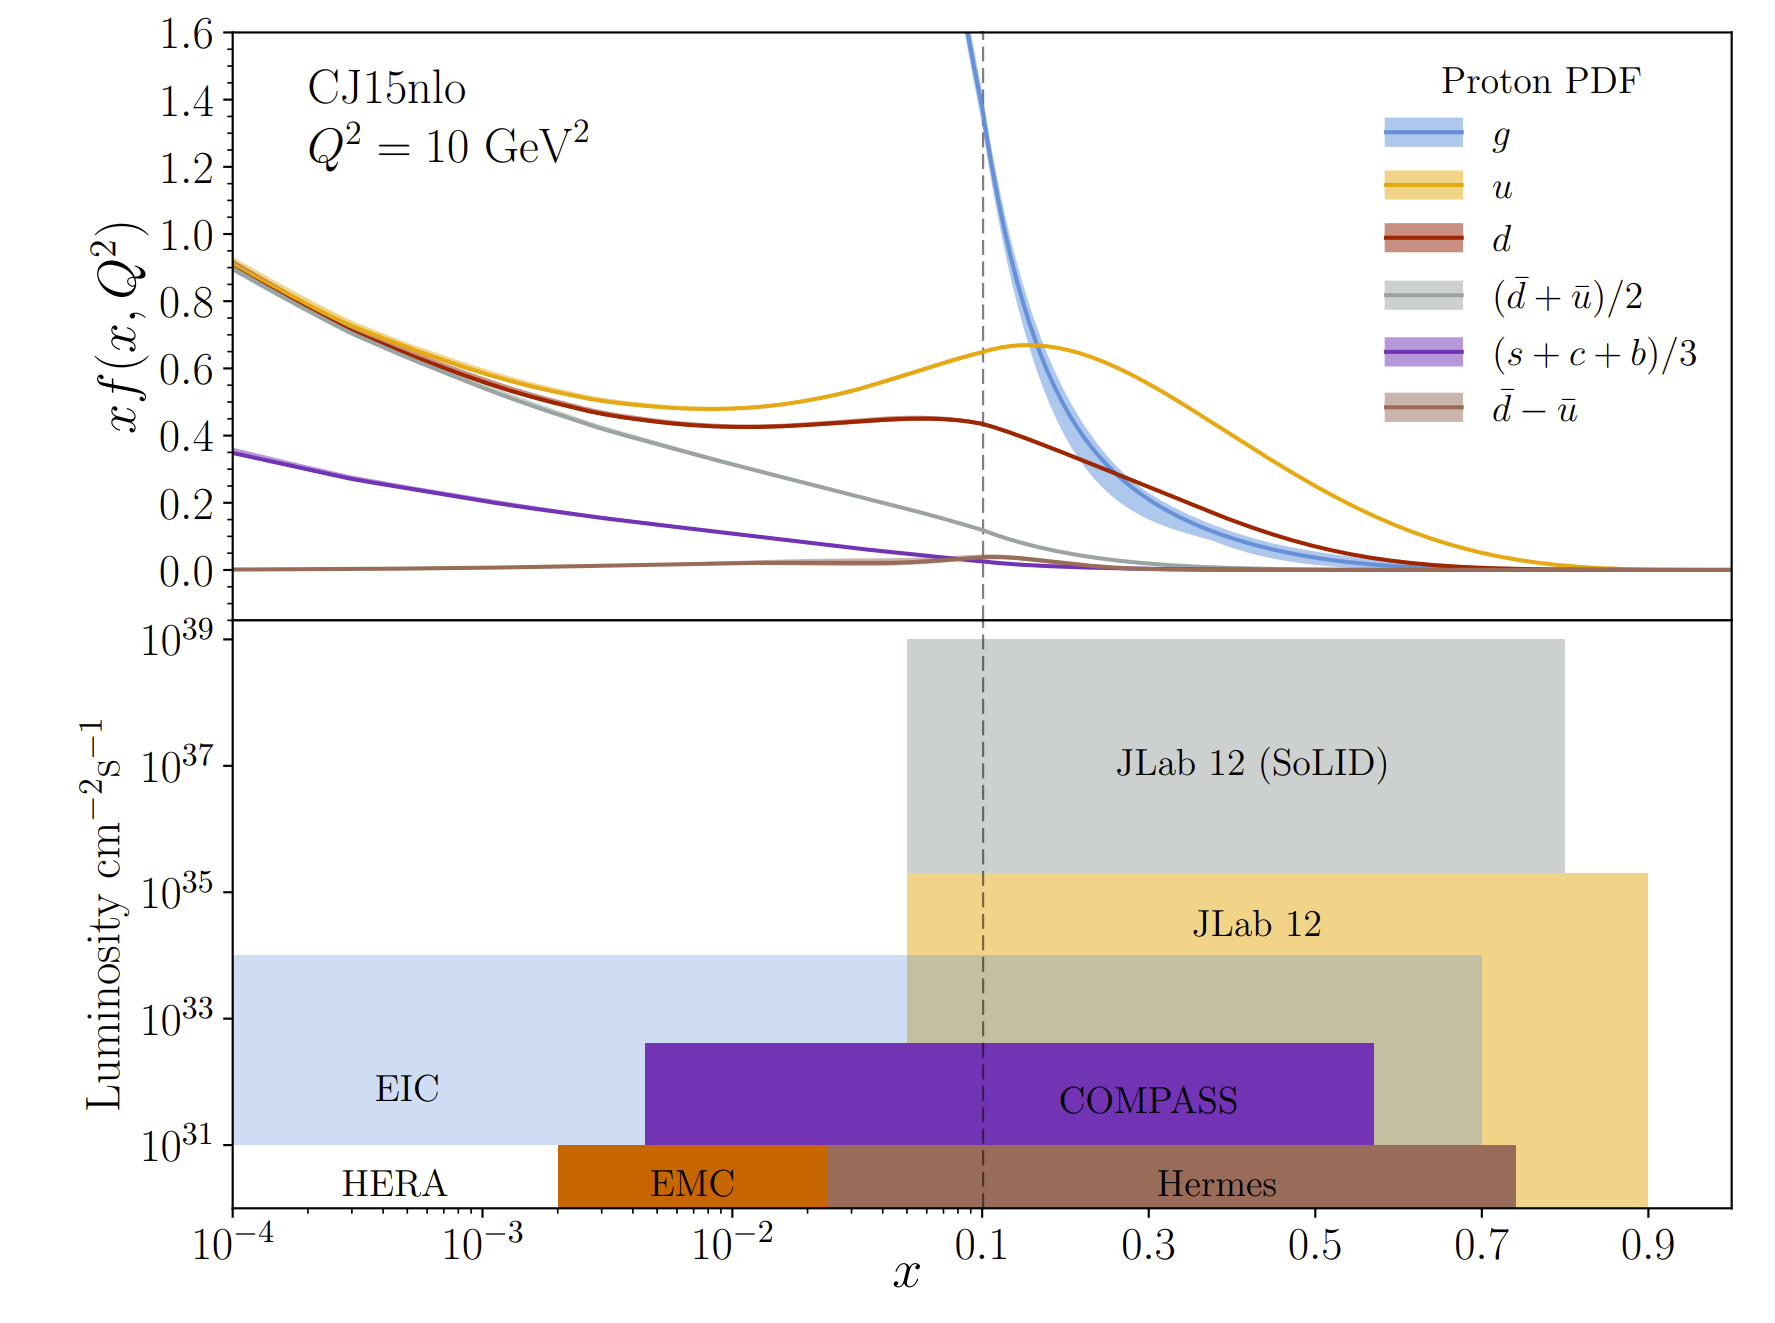
\includegraphics[width=0.9\textwidth]{Chapters/Ch5-Further/X_conclusion/pics/future.png}
    \caption[Kinematic Overlap of Future Experiments]{Kinematic regions of Deep Inelastic Scattering and the comparative reach of EIC and CEBAF, from \parencite{Arrington2022PhysicsOpportunities} }
    \label{fig:physics_future_ranges}
\end{figure}
